\documentclass[a4paper]{article}
\usepackage[utf8]{inputenc}
\usepackage[spanish, es-tabla]{babel}

\usepackage{amsmath}
\usepackage{amsfonts}
\usepackage{amssymb}

\usepackage{float}
\usepackage{graphicx}
\graphicspath{ {./Imagenes/} }

\usepackage{multirow}
\setlength{\doublerulesep}{\arrayrulewidth}

\usepackage{array}
\newcolumntype{C}[1]{>{\centering\let\newline\\\arraybackslash\hspace{0pt}}m{#1}}

\usepackage[american]{circuitikz}

\usepackage{fancyhdr}

\usepackage{units} 

\pagestyle{fancy}
\fancyhf{}
\lhead{22.02 Electrotecnia I}
\rhead{Mechoulam, Mestanza, Lambertucci, Pouthier, Londero}
\rfoot{Página \thepage}



\begin{document}

%%%%%%%%%%%%%%%%%%%%%%%%%%%%%%%%%%%%%%%%%%%%%%%%%%%%%%%%%%%%%%%%%%%%%%%%% 
%								CARATULA								%
%%%%%%%%%%%%%%%%%%%%%%%%%%%%%%%%%%%%%%%%%%%%%%%%%%%%%%%%%%%%%%%%%%%%%%%%% 

\begin{titlepage}
\newcommand{\HRule}{\rule{\linewidth}{0.5mm}}
\center
\mbox{\textsc{\LARGE \bfseries {Instituto Tecnológico de Buenos Aires}}}\\[1.5cm]
\textsc{\Large 22.02 Electrotecnia I}\\[0.5cm]


\HRule \\[0.6cm]
{ \Huge \bfseries Trabajo práctico N$^{\circ}$3}\\[0.4cm] 
\HRule \\[1.5cm]


{\large

\emph{Grupo 5}\\
\vspace{3px}

\begin{tabular}{lr} 	
\textsc{Mechoulam}, Alan  &  58438\\
\textsc{Lambertucci}, Guido Enrique  & 58009 \\
\textsc{Pouthier}, Florian  & 61337 \\
\textsc{Mestanza}, Nicolás  & 57521 \\
\textsc{Londero Bonaparte}, Tomás Guillermo  & 58150 \\
\end{tabular}

\vspace{20px}

\emph{Profesores}\\
\vspace{3px}
\textsc{Muñoz}, Claudio Marcelo\\ 	
\textsc{Ayub}, Gustavo\\ 	

\vspace{100px}

\begin{tabular}{ll}

Presentado: & 17/05/19\\

\end{tabular}

}

\vfill

\end{titlepage}


%%%%%%%%%%%%%%%%%%%%%%%%%%%%%%%%%%%%%%%%%%%%%%%%%%%%%%%%%%%%%%%%%%%%%%%%% 
%								INFORME									%
%%%%%%%%%%%%%%%%%%%%%%%%%%%%%%%%%%%%%%%%%%%%%%%%%%%%%%%%%%%%%%%%%%%%%%%%%

\section*{Introducción}

En este trabajo práctico, se somete al análisis a dos cuadripolos, a los cuales se les determinan sus parámetros impedencia [Z], admitancia [Y] y trasmisión [T] y se analizan sus máximas transferencias de potencia. Luego se los pone en serie, paralelo y cascada, y se ensayan aquellos nuevos cuadripolos. Finalmente se comparan los parametros obtenidos de los nuevos cuadripolos y se comparan con los parametros calculados mediante el equivalente teórico a partir de los parametros de los cuadripolos originales.

\section*{Desarrollo de la experiencia}

Los cuadripolos asignados al grupo son:
\begin{enumerate}
	\item[A)] Número de serie: 9603, de disposición tipo Pi;
	\item[B)] Número de serie: 9608, de disposición tipo T.
\end{enumerate}
ambos de tensión y corriente máxima de $15 \ V$ y $50 \ mA$. Cabe aclarar que se consideró $I_2$ saliente, por lo tanto, se cambió el signo de los parametros B y D.

De las mediciones se obtuvo:

\begin{table}[H]
\begin{center}
\begin{tabular}{|c|c|c|c|c|}
\hline
\multicolumn{5}{|c|}{Cuadripolo A - Nro. De serie: - 9603} \\ \hline
 & $V_1 \ [V]$ & $V_2 \ [V]$ & $I_1 \ [mA]$ & $I_2 \ [mA]$ \\ \hline
$V_1 = 0$ & 0 & 3,05 & 41,5 & 30 \\ \hline
$V_2 = 0$ & 3,05 & 0 & 36 & 30,25 \\ \hline
$I_1 = 0$ & 2,56 & 3,05 & 0 & 16,25 \\ \hline
$I_2 = 0$ & 3,05 & 2,20 & 14 & 0 \\ \hline
\end{tabular}
\caption{Mediciones realizadas en el cuadripolo A.}
\end{center}
\end{table}

\begin{table}[H]
\begin{center}
\begin{tabular}{|c|c|c|c|c|}
\hline
\multicolumn{5}{|c|}{Cuadripolo B - Nro. De serie: 9608} \\ \hline
 & $V_1 \ [V]$ & $V_2 \ [V]$ & $I_1 \ [mA]$ & $I_2 \ [mA]$ \\ \hline
$V_1 = 0$ & 0 & 3,05 & 11,5 & 16 \\ \hline
$V_2 = 0$ & 3,05 & 0 & 16,75 & 11,5 \\ \hline
$I_1 = 0$ & 2,11 & 3,05 & 0 & 6,8 \\ \hline
$I_2 = 0$ & 3,05 & 2,19 & 8,2 & 0 \\ \hline
\end{tabular}
\caption{Mediciones realizadas en el cuadripolo B.}
\end{center}
\end{table}

\subsection*{Cálculos}

A partir de los valores medidos antes, se pueden calcular los parámetros correspondientes de cada cuadripolo ensayado.

\begin{equation}
\text{Cuadripolo A :}\quad [Z_{A}] =
\left( \begin{array}{cc}
	217,86 & 157,35\\
	157,36 & 187,69\\
\end{array} \right)
\end{equation}

\begin{equation}
\text{Cuadripolo B :}\quad [Z_{B}] =
\left( \begin{array}{cc}
	371,95 & 310,29\\
	266,46 & 448,53\\
\end{array} \right)
\end{equation}

\begin{equation}
\text{Cuadripolos en serie :}\quad [Z_{Serie}] =
\left( \begin{array}{cc}
	561,82 & 605,88\\
	157,36 & 187,69\\
\end{array} \right)
\end{equation}

\subsubsection*{Parámetros de admitancia Y}

\begin{equation}
\text{Cuadripolo A :}\quad [Y_{A}] =
\left( \begin{array}{cc}
	0,012 & -0,014\\
	-0,010 & 0,010\\
\end{array} \right)
\end{equation}

\begin{equation}
\text{Cuadripolo B :}\quad [Y_{B}] =
\left( \begin{array}{cc}
	0,005 & -0,004\\
	-0,004 & 0,005\\
\end{array} \right)
\end{equation}

\begin{equation}
\text{Cuadripolos en paralelo :}\quad [Y_{Paralelo}] =
\left( \begin{array}{cc}
	0,007 & 0,013\\
	0,013 & 0,002\\
\end{array} \right)
\end{equation}

\subsubsection*{Parámetros de transmisión T}

\begin{equation}
\text{Cuadripolo A :}\quad [T_{A}] =
\left( \begin{array}{cc}
	1,38 & 100,83\\
	0,01 & 1,19\\
\end{array} \right)
\end{equation}

\begin{equation}
\text{Cuadripolo B :}\quad [T_{B}] =
\left( \begin{array}{cc}
	1,40 & 265,22\\
	0,004 & 1,46\\
\end{array} \right)
\end{equation}

\begin{equation}
\text{Cascada A-B :}\quad [T_{A-B}] =
\left( \begin{array}{cc}
	2,29 & 515\\
	0,01 & 3,42\\
\end{array} \right)
\end{equation}

\begin{equation}
\text{Cascada B-A :}\quad [T_{B-A}] =
\left( \begin{array}{cc}
	3,56 & 468,18\\
	0,02 & 2,20\\
\end{array} \right)
\end{equation}

\subsection*{Equivalencia de parámetros de cuadripolos individuales}

A continuación, se verificará la correspondencia entre los valores medidos y los valores calculados con diferentes fórmulas conocidas.

\subsubsection*{Equivalencia [Z] - [Y]}

Calculando Z, para cada cuadripolo, mediante la formula relación $[Z]=[Y]^{-1}$, se observa:

\begin{equation}
\text{Cuadripolo A :}\quad [Z_{Teorico}] =
\left( \begin{array}{cc}
	-521,74 & -721,74\\
	-500,09 & -626,09\\
\end{array} \right)
\end{equation}

\begin{equation}
\text{Cuadripolo B :}\quad [Z_{Teorico}] =
\left( \begin{array}{cc}
	359,48 & 258,38\\
	 258,34 & 376,34\\
\end{array} \right)
\end{equation}

\subsubsection*{Equivalencia [Z] - [T]}

De forma análoga, se calcula T mediante los valores medidos de Z, considerando la $I_2$ saliente: 

\begin{equation}
\text{Cuadripolo A :}\quad [T_{Teorico}] =
\left( \begin{array}{cc}
	1,384 & 102,502\\
	0,006 & 1,193\\
\end{array} \right)
\end{equation}

\begin{equation}
\text{Cuadripolo B :}\quad [T_{Teorico}] =
\left( \begin{array}{cc}
	1,396 & 315,800\\
	0,004 & 1,683\\
\end{array} \right)
\end{equation}

\subsection*{Equivalencia de parámetros de cuadripolos asociados}

Por último, se calculan los parámetros medidos en la primer instancia, de las conexiones serie, paralelo y cascada:

\begin{equation}
\text{Conexión Serie :}\quad [Z_{Teorico}] =
\left( \begin{array}{cc}
	589,81 & 467,65\\
	423,82 & 636,22\\
\end{array} \right)
\end{equation}

\begin{equation}
\text{Conexión Paralelo :}\quad [Y_{Teorico}] =
\left( \begin{array}{cc}
	0,017 & -0,017\\
	-0,014 & 0,015\\
\end{array} \right)
\end{equation}

\begin{equation}
\text{Conexión Cascada A - B :}\quad [T_{Teorico}] =
\left( \begin{array}{cc}
	2,317 & 609,76\\
	0,013 & 4,02\\
\end{array} \right)
\end{equation}

\begin{equation}
\text{Conexión Cascada B - A :}\quad [T_{Teorico}] =
\left( \begin{array}{cc}
	3,92 & 519,76\\
	0,016 & 2,39\\
\end{array} \right)
\end{equation}

\section*{Transferencia de potencia máxima}
Se midió la resistencia a la salida de cada cuadripolo, determinando a si la resistencia de Thevenin de cada uno. De esta forma se asentó que $Z_{Th}(A) = 188,3 \ \Omega$ y $Z_{Th}(B) = 383 \ \Omega$. Luego se determinó la corriente y la tension del secundario, variando la resistencia de carga. De esta forma se obtuvieron, para cada cuadripolo, los siguientes valores:

\begin{figure}[H]
	\centering
	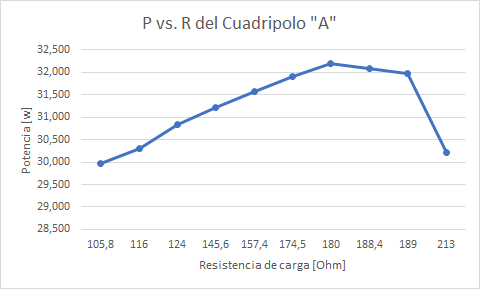
\includegraphics[width=0.8\textwidth]{Potencia-A}
	\caption{Potencia en función de la resistencia de carga del cuadripolo 9603.}
	\label{fig:PA}
\end{figure}

\begin{figure}[H]
	\centering
	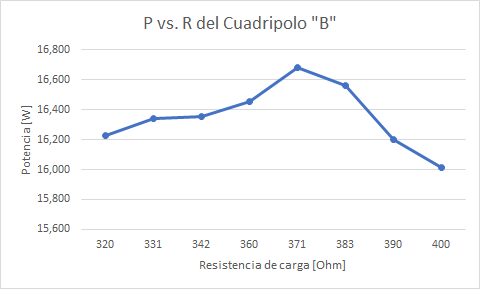
\includegraphics[width=0.8\textwidth]{Potencia-B}
	\caption{Potencia en función de la resistencia de carga del cuadripolo 9608.}
	\label{fig:PB}
\end{figure}

\section*{Conclusión}

En la primer instancia del trabajo se pueden observar varias discrepancias importantes entre los valores medidos y los calculados, como es en los casos de $Z_A$ y de $Y_Paralelo$. Se atribuye dichas diferencias a errores propios de los cuadripolos.
En la segunda instancia, se obtuvieron los valores esperados, acordes a las impedancias de Thevenin de cada cuadripolo.

\end{document}
